\documentclass[10pt,twocolumn,letterpaper]{article}

\usepackage{cvpr}
\usepackage{times}
\usepackage{epsfig}
\usepackage{graphicx}
\usepackage{amsmath}
\usepackage{amssymb}
\usepackage{float}


% Include other packages here, before hyperref.

% If you comment hyperref and then uncomment it, you should delete
% egpaper.aux before re-running latex.  (Or just hit 'q' on the first latex
% run, let it finish, and you should be clear).
\usepackage[pagebackref=true,breaklinks=true,letterpaper=true,colorlinks,bookmarks=false]{hyperref}

\cvprfinalcopy % *** Uncomment this line for the final submission

\def\cvprPaperID{} % *** Enter the CVPR Paper ID here
\def\httilde{\mbox{\tt\raisebox{-.5ex}{\symbol{126}}}}


% Pages are numbered in submission mode, and unnumbered in camera-ready
\ifcvprfinal\pagestyle{empty}\fi
\begin{document}

%%%%%%%%% TITLE
\title{Salient Point Reduction for Content-Based Image Retrieval}

\author{Yao-Hong Tsai}

\maketitle
%\thispagestyle{empty}

%%%%%%%%% ABSTRACT
\begin{abstract}

	Salient points are frequently used to represent local properties of the 
	image in content-based image retrieval.In this paper, We present a reduction
	algorithms that extracts the local most salient points such that they not give
	a satistying representation of an image,but also make the image retrieval process
	efficeiently. This algorithm recurisvely reduces the continuous point set by 
	their corresponding saliency values under a top-down approach. 
	The resulting salient points are evaluated with an image retrival system 
	using Hausdoff distance. In this experiment, it shows that our method
	is robust and the extracted salient points provide better retrieval
	performance comparing with other point detectors.
   
\end{abstract}

%%%%%%%%% BODY TEXT

\section{Math formula}
\begin{equation}
	S=\sum_{k=1}^{-j}\left | C^{k}(W_{2^{j}}f(m,n)) \right |
\end{equation}
	For a point in an image, its corresponding saliency value is
	computed for every wavelet coefficient. We then have to
	threshold the saliency value, in relation to the desired number
	of salient points. 
% ------------------------------------------------------------------------
\section{image}

	\begin{table}[H]
	\begin{center}
	\begin{tabular}{|l|c|}
	\hline
	Method & Frobnability \\
	\hline\hline
	1 & \\
	2 & \\
	3 & \\
	4 & \\
	\hline
	\end{tabular}
	\end{center}
	\caption{}
	\end{table}
%------------------------------------------------------------------------
\section{table}

	\begin{figure}[H]
	\begin{center}
	   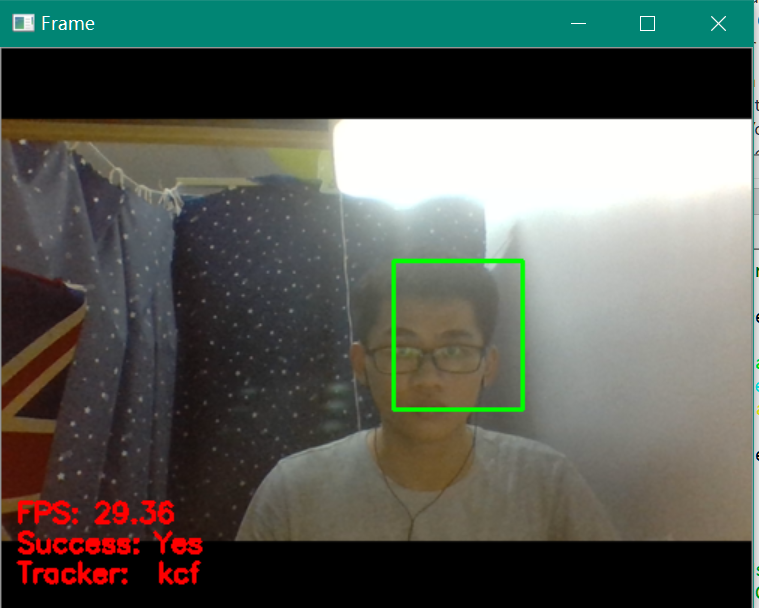
\includegraphics[width=0.8\linewidth]{1.png}
	\end{center}
	   \caption{ Results of the CBIR using salient points generated by
	Song’s algorithm.}
	\label{img3}
	\end{figure}
%------------------------------------------------------------------------
\section{citation}

Here is a exemple of citation\cite{Fiala2006Using}.

{\small
\bibliographystyle{ieee_fullname}
\bibliography{egbib}
}


\end{document}
